\documentclass{report}
\usepackage{pgfplots}


\input{preamble}
\input{macros}
\input{letterfonts}


\title{\Huge{Travaux dirigées}\\ Ensembles}
\author{\huge{A.Belcaid}}
\date{\today}

\begin{document}

\maketitle
\newpage% or \cleardoublepage
% \pdfbookmark[<level>]{<title>}{<dest>}
\pdfbookmark[section]{\contentsname}{toc}
\tableofcontents
\pagebreak

\chapter{}
\section{Exercice 1}
% Exercise 1 {{{ %
\qs{}{
Montrer que $\emptyset \subset X$, pour tout ensemble $X$.
}

\begin{myproof}
  On procède par  \textbf{contraposition}: \\

  On suppose alors 
  $$
  \exists X \subset E\; |\; \emptyset \not \subset X
  $$
  Ce qui se traduit par:
  $$
  \exists x \in \emptyset \text{ et } x \not\in X
  $$
  Ce qui est absurde car l'expression $ x \in \emptyset$ est toujours
  \textbf{fausse}.

\end{myproof}


% }}} Exercise 1 %
% Exercise 2 {{{ %

\section{Exercice 2}

\qs{}{
  Soit $E$ un ensemble donné et soient $A,B \in \mathcal{P}(E)$,  montrer par contraposition les assertions suivantes:
\begin{enumerate}
\item $(A\cap B=A\cup B)\Rightarrow A=B$,
\item $ (A\cap B=A\cap C \text{ et } A\cup B=A\cup C)\implies B=C$.
\end{enumerate}
}
\begin{myproof}
\begin{enumerate}
  \item On procède la aussi par \textbf{contraposition}. On suppose alors que
    $A\neq B$ et on démontre que $A\cap B \neq A \cup B$.\\

    Puisque $A \neq B$, on peut supposer (\textbf{sans perte de généralité}) que:

       $$
       \exists x \in A \; \text{ et } x \not\in B
       $$
  
       \nt{En cas contraire,  on peut permuter le rôle de $A$ et $B$ et la démonstration reste la même.}
       Ainsi 
       $$ x \in A\cup B  \quad {et} \quad x \not\in A \cap B$$
       Ce qui prouve que: 

       $$
       A\cup B \neq A \cap B
       $$
     \item Pour la deuxième partie de la question:
       On suppose que $A\cap B=A\cap C \text{ et } A\cup B=A\cup C$ et on
       démontre que $B = C$.

       \begin{enumerate}
         \item On commence par la première inclusion $ B \subset C$.\\

           Soit alors $x \in B $.
           Alors on doit traiter deux cas:

           \begin{enumerate}
           \item $x \in A \implies x \in A\cap B = A\cap C \implies x\in C$ 
           \item $x\not\in A \text{ et } x\in A\cup B = A\cup C$.\\
             puisque $x\not\in A$ et $x\in A\cup C$ on conclut forcement que $x \in C$.
           \end{enumerate}
         \item L'inclusion inverse suit le même processus.
       \end{enumerate}
\end{enumerate}
\end{myproof}

% }}} Exercise 2 %
% Exercise 3 {{{ %

\section{Exercice 3}
\qs{}{
Soient $E$ et $F$ deux ensembles et $f:E\rightarrow F$ une application de $E$ vers $F$.\\

Démontrer que:

\begin{itemize}
  \item $\forall A,B \in \mathcal{P}(E) \quad (A\subset B)\Rightarrow (f(A)\subset f(B))$
  \item $\forall A,B \in \mathcal{P}(E) \quad f(A\cap B)\subset f(A)\cap f(B)$
  \item $\forall A,B \in \mathcal{P}(E) \quad f(A\cup B) = f(A)\cup f(B)$
  \item $\forall A,B \in \mathcal{P}(F) \quad f^{-1}(A\cup B) = f^{-1}(A)\cup f^{-1}(B)$
  \item $\forall A \in \mathcal{P}(F) \quad f^{-1}(F\setminus A)=E\setminus f^{-1}(A)$
\end{itemize}
}
\begin{myproof}
 \begin{enumerate}
   \item On suppose que $A\subset B$  et on demontre que  $f(A)\subset f(B)$.\\

     Soit $y\in f(A) \implies \exists x \in A \; \text{tel que } y = f(x)$
     Comme $A\subset B$, on conclut alors que:
     $$
     \exists x \in B\; \text{ tel que } y = f(x) \implies y \in f(B)
     $$
     Ainsi
     $$
     f(A) \subset f(B).
     $$
   \item On démontre que $f(A\cap B) = f(A)\cap f(B)$.\\

     Soit alors $y \in f(A\cap B) \implies \exists y \in A\cap B \;\text{tel que } y = f(x)$.\\

     On conclut que

     $$
     \begin{cases}
       \exists x \in A \; \text{tel que } y = f(x) &\implies y \in f(A). \\[4pt]

       \exists x \in B \; \text{tel que } y = f(x) &\implies y \in f(B). \\

     \end{cases}
     $$
     Ainsi on conclut que 
     $$
     y \in f(A) \cap f(B)
     $$

  \item  On procède par double inclusion:\\
    \begin{enumerate}
      \item On demontre que $f(A\cup B) \subset f(A)\cup f(B)$.\\

        Soit alors $y\in f(A\cup B) \implies \exists x \in A\cup B \; \text{tel
        que } y = f(x)$.\\

        Étant le rôle symétrique que joue $A$ et $B$, on peut supposer
        \textbf{sans perte de généralité} que 

        $$
        x\in A \implies y \in f(A) \implies y \in f(A)\cup f(B)
        $$

  \item On démontre que  $ f(A)\cup f(B) \subset f(A\cup B)$.
    Soit alors 

    $$
    y\in f(A)\cup f(B)
    $$
    Ainsi on aura que 
    $$
    \begin{cases}
      \exists x \in A \; \text{tel que } &y = f(x)\\
      \text{ou} & \\
      \exists x \in B \; \text{tel que } &y = f(x)\\
    \end{cases}
    $$
    on conclut alors que 
    $$
    \exists x \in A\cup B \; \text{tel que } y = f(x) \implies y \in f(A\cup B)
    $$
    \end{enumerate}
    On utilise la simple définition:
    \begin{eqnarray*}
      f^{-1}(A\cup B) &=&  \left\{ x \in E \; \text{tel que } f(x) \in A \cup
      B\right\}\\
                      & = & \left\{x \in E \; \text{tel que } f(x) \in A \text{
                        ou } f(x) \in B\right\}\\
                        &=& \left\{x\in E \;\text{ tel que } f(x) \in A \right\}
                        \cup \left\{x\in E \;\text{ tel que } f(x) \in B
                        \right\}\\
                        &= & f^{-1}(A) \cup f^{-1}(B)
    \end{eqnarray*}
    
  \item
    On as 
    \begin{eqnarray*}
      f^{-1}(F\backslash A) & = &\left\{x\in E\;\text{tel que } f(x) \not\in
      A\right\}\\[4pt]
                            &=& \overline{\{x\in E\;\text{tel que } f(x)\in
                            A\}}\\[4pt]
                            &=& E \backslash f^{-1}(A)
    \end{eqnarray*}
\end{enumerate}

  
\end{myproof}


% }}} Exercise 3 %
% Exercise 4 {{{ %
\section{Exercice 4}

\qs{}{

Soit $E$ un ensemble et $A, B, C$ trois parties de $E$.\\
Montrer que
$$ (A \cup B) \cap (B \cup C) \cap (C \cup A) =
(A \cap B) \cup (B \cap C) \cup (C \cap A)$$
}
\begin{myproof}
  \begin{eqnarray*}
    (A \cup B) \cap (B \cup C) \cap (C \cup A) &=& \big[(A\cap B)\cup
    (A\cap C)\cup(B \cap B )\cup (B \cap C)\big] \cap( C\cup A)\\
                                               &=&
                                               (A\cap B\cap C)\cup (A\cap B)\cup
                                               (B\cap C)\cup (A\cap C)\\
                                               &=&(A \cap B) \cup (B \cap C) \cup (C \cap A)
  \end{eqnarray*}

\end{myproof}
\nt{Dans la deuxième ligne de l'équation, on a élimine des ensembles redondants
comme
$$
(A\cap B) \cup (A\cap B) = (A\cap B)
$$
}


% }}} Exercise 4 %

% Exercice 5 {{{ %
\vspace*{0.4cm}
\section{Exercice 5}
\qs{}{
Montrer que si $F$ et $G$ sont des sous-ensembles de $E$~:
\begin{enumerate}
  \item $(F \subset G \iff F \cup G = G )$
  \item $(F \subset G \iff \complement F \cup G = E).$
\end{enumerate}
En déduire que~: 
\begin{enumerate}
  \item $ (F \subset G \iff F \cap G = F)$
  \item $(F \subset G \iff F \cap\complement G = \emptyset).$ 
\end{enumerate}
}
\begin{myproof}

 \begin{enumerate}
   \item  On démontre la premier eh implication:\\

   \begin{itemize}
     \item On suppose que $F\subset G$. On sait deja que pour n'importe quel
       deux ensembles on $G \subset F\cup G$. On prend alors un $x \in F\cup G
       \implies \{x \in F \text{ ou } x\in G\}\implies
       \{x \in G \text{ ou } x\in G\}\implies 
       x \in G.$.
       Ainsi on conclut que
       $$
       F\subset G \implies F\cup G = G
       $$
     \item \textbf{Implication inverse}: On suppose que $F\cup G = G$.\\

       Soit alors $x \in F\implies x\in \underbrace{F\cup G}_{G} \implies x\in G$
       
   \end{itemize}
   
     \item De même on procède par double implication. 
       \begin{itemize}
         \item \textbf{On suppose que } $F\subset G$.
           On a deja que $\complement F \cup G \subset E$ pour n'importe quel
           deux ensembles dans $E$. On demontre alors l'inclusion inverse:\\

         Soit $x \in E\implies x\in G \text{ ou } x\not\in G\implies x \in G
         \text { ou } x\in \complement G $\\
      et puisque $F\subset G \implies \complement G \subset \complement F$.
      On conclut alors que $$ x \in G \text { ou } x \in \complement F$$

       \end{itemize}

   
 \end{enumerate}

 Pour la deuxième partie on utilise les premiers résultats.

 \begin{enumerate}
   \item On a $$
     F \subset G \iff \complement G \subset \complement
     F\underbrace{\iff}_{\text{1}} \complement G \cup \complement F = \complement
     F \iff G \cap F = F
     $$
   \item 
     $$
     F \subset G \underbrace{\iff}_{2} \complement F \cup G = E
     \underbrace{\iff}_{\text{morgan}} F \cap \complement G = \emptyset
     $$
 \end{enumerate}
  
\end{myproof}
% }}} Exercice 5 %

% Exercie 6 {{{ %
\section{Exercice 6} 
\qs{}{ Soit $A= \{a_1, a_2, a_3, a_4\}$ et $B= \{b_1, b_2, b_3, b_4 ,b_5\}$. \begin{itemize} \item Écrire le produit cartésien $A \times B$. \item Quel est le nombre de parties de $A \times B$~? \end{itemize} }
\begin{myproof}
  
  \begin{itemize}
    \item 
      $$
      A\times B = \{(a_i, b_j)\; |\;  1\leq i \leq 4 \text{ et } 1 \leq j \leq 5\}
      $$
      \nt{On peut aussi lister tous les couples qui ont un cardinal de
      $\mathbf{20}$}
    \item Le nombre de parties d'un ensemble de cardinal $n$ est $2^n$. Ainsi 
      $$
      \mathcal{C}ard\big(\mathcal{P}(A \times B)\big) = 2^{20}
      % \mathcal{C}ard{\mathcal{P}(A\times B) = 2^{20}
      $$
  \end{itemize}
\end{myproof}



% }}} Exercie 6 %

% Exercice 7 {{{ %
\section{Exercice 7}
\qs{}
{

Soit $A\subset E$, on appelle fonction caractéristique de~$A$
l'application~$f$ de~$E$ dans l'ensemble à deux éléments $\{0, 1\}$, telle
que~:
$$f(x)=\begin{cases}
0&  \text{ si } x\notin A \cr 1& \text{ si } x \in A \cr
\end{cases}$$
Soient $A$ et $B$ deux parties de $E$, $f$ et $g$ leurs fonctions
caractéristiques.\\
Montrer que les fonctions suivantes sont les fonctions
caractéristiques d'ensembles que l'on déterminera~:
\begin{enumerate}
\item $1-f$.
\item $fg$.
\item $f+g-fg$.
\item $f + g - 2fg$
\end{enumerate}

}
\begin{myproof}
  
  Je vais utiliser la notation $\varPi_A$ pour dénoter la fonction
  \textbf{caractéristique} d'un ensemble $A$. Ainsi $f=\varPi_A$ et $g=\varPi_B$.
  \begin{enumerate}
      \item 
      $$
     1 - f = \varPi_A = \begin{cases}
      1 - 1 & x \in A   \\
      1 - 0 & x \not\in A
    \end{cases} = 
\begin{cases}
  0 & x \notin \overline{A}   \\
  1  & x \in \overline{A}
\end{cases} = \varPi_{\overline{A}}
      $$
    \item De même on trouve que
      $$
      fg = \varPi_A\;\varPi_B = \varPi_{A\cap B}.
      $$
    \item 
      $$
      f + g - fg\; =\; \varPi_A + \varPi_B - \varPi_A\;\varPi_B\; =\; \varPi_{A \cup B}
      $$
    \item 

      $$
      f + g - 2fg\; =\; \varPi_A + \varPi_B - 2\varPi_A\;\varPi_B\; =\;
      \varPi_{A \Delta B}
      $$
  \end{enumerate}
  
\end{myproof}
% }}} Exercice 7 %

% Exercice 8 {{{ %
\section{Exercice 8}

\qs{}
{
Soit un ensemble $E$ et deux parties $A$ et $B$ de~$E$. 
\begin{enumerate}
\item Démontrer que $A \triangle B = (A \setminus B) \cup(B \setminus A)$.
\item Démontrer que pour toutes les parties $A$, $B$, $C$ de $E$ on a
$(A \bigtriangleup B) \bigtriangleup C = A \triangle(B \triangle C)$.
\item Démontrer qu'il existe une unique partie~$X$ de~$E$ telle que 
pour toute partie~$A$ de~$E$, $A \triangle X = X \triangle A = A$.
\item Démontrer que pour toute partie $A$ de $E$, il existe une partie~$A'$
de~$E$ et une seule telle que $$A \triangle A' = A' \triangle A = X$$.

\textit{ \textbf{Indice:}  \scriptsize Il pourra être commode 
d'utiliser la notion de fonction caractéristique.}
\end{enumerate}
}
\begin{myproof}
  
  Par définition du cours on as :
  $$
  A \triangle B = (A\cup B) \backslash (A\cap B)
  $$
  \begin{enumerate}
    \item 
      \begin{eqnarray*}
        A \triangle B &=& \left\{  x \in E \;|\; x \in (A\cup B) \text{ et } x
          \not\in
        (A\cap B)\right\} \\
        &=&\left\{  x \in E \;|\; \big(x \in A \text{ et } x \not\in
        (A\cap B)\big)\text{ ou } 
\big(x \in B \text{ et } x \not\in
        (A\cap B)\big)
      \right\}\\
        &=&\left\{  x \in E \;|\; \big(x \in A \text{ et } x \not\in
        B\big)\text{ ou } 
\big(x \in B \text{ et } x \not\in
        A\big)
      \right\}\\
        &=& (A\backslash B) \cup (B \backslash A)
      \end{eqnarray*}
  \end{enumerate}
  
\item On reprend la première question mais cette fois en utilisant la notion de
  fonction \textbf{caractéristique}: On admet que 
  $$
  \varPi_A = \varPi_B \iff A = B
  $$
  \nt{Ce qui veut dire que l'égalité des fonctions caractéristiques est
  équivalente a l'égalité des ensembles. Ainsi pour démontrer que deux ensembles
sont égales, il suffit de démonter que leurs fonctions caractéristiques sont
égales.}
On a déjà établi que 
\begin{itemize}
  \item $\varPi_{\overline{A}} = 1 - \varPi_A$\\
  \item $\varPi_{A\cap B} = \varPi_A \varPi_B $.\\
  \item $\varPi_{A\cup B } = \varPi_A + \varPi_B - \varPi_{A\cap B}$.\\
  \item $\varPi_{A\Delta B } = \varPi+{A} + \varPi_{B} -2\varPi_{A}\varPi_{B}$
\end{itemize}
Il nous reste alors an en déduire la fonction caractéristique de $A \backslash
B$. Puisque 

\begin{eqnarray*}
  A \backslash B = A \cap \overline{B} 
\end{eqnarray*}

On conclut que 
\begin{eqnarray*}
  \varPi_{A\backslash B}& =&  \varPi_A \; \varPi_{\overline{B}}\\
                        &=& \varPi_A \left( 1 - \varPi_B\right)\\
                        &=& \varPi_A - \varPi_A\varPi_B
\end{eqnarray*}

 Il suffit maintenant de prouver que 
 $$
 \varPi_{(A\backslash B) \cup (B\backslash A)} = \varPi_A + \varPi_B -
2\varPi_A\varPi_B
 $$
On procède par les relations établies:
\begin{eqnarray*}
  \varPi_{ (A\backslash B) \cup (B\backslash A)}  &=& \varPi_{A\backslash B} +
  \varPi_{B\backslash A}  - \varPi_{A\backslash B}\varPi_{B\backslash A}\\
                                                  &=&
                                                  \varPi_A -\varPi_A\varPi_B +
                                                  \varPi_B - \varPi_{A\backslash
                                                  B}\varPi_{B\backslash A}\\
                                                  &=&
                                                  \varPi_A -\varPi_A\varPi_B +
                                                  \varPi_B - \left(\varPi_A -
                                                  \varPi_{A}\varPi_B\right)\left(\varPi_B
                                                - \varPi_A\varPi_B\right)\\
                                                  &=& \varPi_A + \varPi_B -
                                                  2\varPi_A\varPi_B 
\end{eqnarray*}

\end{myproof}

\nt{
  Dans le calcul de la derrières ligne on utilise l'astuce que
  $$
  \varPi_A\varPi_B \varPi_A = \varPi_{A\cap B \cap A} = \varPi_{A \cap B} =
\varPi_A \varPi_B
  $$
}

\begin{myproof}
  \begin{itemize}
    \item On procède par fonction caractéristique pour calculer 
      $$
      \varPi_{(A \triangle B )\triangle C} \text{ et } \varPi_{A \triangle ( B
      \triangle C)}. 
      $$
    \item
      \begin{itemize}
        \item \textbf{Existence}
          On sait que 
          $$
          \forall A \subset E \quad A \triangle \emptyset = \emptyset \triangle A
          =  (A\cup \emptyset) \backslash (A \cap \emptyset)  = A \backslash
          \emptyset = A
          $$
        \item \textbf{Unicité}
          On suppose qu'il existe un ensemble $B \ne \emptyset$ tel que:
          $
A \triangle B = B \triangle A = A
$
Puisque $B \ne \emptyset$ soit alors $x \in B$.
 On as deux cas:
 \begin{enumerate}
   \item $x\in A \implies x \not\in A\triangle B \implies x \not \in A$. Absurde.
   \item $x\not\in A \implies x \in A\triangle B \implies x \in A$. Absurde
 \end{enumerate}

 Ainsi $\emptyset$ est l'\textbf{unique} élément neutre de la différence
 symétrique.

      \end{itemize}
    \item  
      \begin{itemize}
        \item \textbf{Existence}
          $$
          \forall A \subset E \quad A \triangle A = (A\cup A) \backslash (A \cap
          A) = A \backslash A = \emptyset
          $$
        \item \textbf{Unicité}
          On suppose qu'il existe un ensemble $B \ne A$. tel que 
          $$
          A\triangle B = B \triangle A = \emptyset
          $$
        Puisque $$B\ne A \implies \exists x \in B \text{ et } x \not\in A\implies
        x \in B\backslash A \implies x \in A \triangle B = \emptyset$$.\\
        Ce qui est absurde.
      \end{itemize}
  \end{itemize}
\end{myproof}

% }}} Exercice 8 %

% Exercice 9 {{{ %
\section{Exercice 9}
\qs{}
{
Soient $A, B \subset E$.\\
R\'esoudre les \'equations \`a l'inconnue $X \subset E$
\begin{enumerate}
\item $A \cup X = B$.
\item $A \cap X = B$.
\end{enumerate}
}
\begin{myproof}
 Traitons d'abord la première équation. Puisque $A\subset A\cup X$. Une telle
 équation ne peut avoir une solution que si $A\subset B$. Supposons donc cette
 condition \textbf{remplie}.\\
 On détermine alors toutes les solutions. Supposons d'abord que $X$ est une
 solution. Puisque $X\subset A\cup X$, on a nécessairement $X\subset B$. De
 plus, $X$ doit nécessairement contenir tous les éléments de $B$ qui ne sont pas
 dans $A$. Autrement dit
 $$
 B\backslash A \subset X \ \subset B
 $$
 Réciproquement, soit $X$ une partie de $\mathcal{P}(E)$ telle que 
 $$
 B\backslash A \subset X \subset B \implies A\cup X \subset B\cup B = B
 $$
 De plus on as 
 $$
 B = A \cup(B\backslash A) \subset A\cup X
 $$
 On conclut alors que 
 $$
 A \cup X = B
 $$
 \nt{
   Dans toutes les solutions sont les parties $X$ tel que 
   $$
   B\backslash A \subset X \subset B.
   $$
 }
 La deuxième équation se traite de façon similaire puisque on peut revenir a la
 première Question en appliquant le \textbf{complémentaire}.
 On trouve la solution $X$ doit vérifier:

 $$
 B \subset X \subset (B\cup \overline{A}).
 $$
\end{myproof}

% }}} Exercice 9 %

% Exercice 10 {{{ %{{{
\section{Exercice 10}
\qs{Composition}
{
  Soient $f : \mathbb{R} \rightarrow \mathbb{R}$ et $g : \mathbb{R} \rightarrow
  \mathbb{R}$ telles que $f(x) =
3x+1$ et $g(x)=x^2-1$.
\begin{itemize}
  \item  A-t-on $f\circ g=g\circ f\;$?
\end{itemize}

}
\begin{myproof}
  \begin{enumerate}
\item On calcule $f\circ g$. 
  $$
  \forall x \in \mathbb{R}\quad \left(f\circ g\right)(x) = f(x^2 -1) = 3x^2 -2
  $$
\item  De même on calcule l'expression de $g\circ f$.

  $$
  \forall x \in \mathbb{R}\quad \left(g\circ f\right)(x) = g(3x+1) = 9x^2 + 6x
  $$
  \end{enumerate}
  Ainsi on conclut que 
  $$
  \left(f \circ g \right) \neq \left(g \circ f\right)
  $$
\end{myproof}

\nt{Le but de l'exercice est d'inciter que la composition de fonctions n'est pas
\textbf{commutative}}
% }}} Exercice 10 %}}}


% Exercice 11 {{{ %
\newpage
\section{Exercice 11}
\qs{}{
Soit l'application de $\mathbb{R}$ dans $\mathbb{R}$, 
$f\colon x\mapsto x^2$.
\begin{enumerate}
\item Déterminer les ensembles suivants:
  \begin{itemize}
    \item $f([-3,-1])$
    \item $f([-2,1])$
    \item $f([-3,-1]\cup[-2,1])$
    \item $f([-3,-1]\cap[-2,1])$
  \end{itemize}
   
\item Mêmes questions avec les ensembles:
  \begin{itemize}
    \item $f^{-1}(\mathopen]-\infty,2])$
    \item $f^{-1}([1,+\infty\mathclose[)$
    \item $f^{-1}(\mathopen]-\infty,2]\cup\nolinebreak{}[1,+\infty\mathclose[)$
    \item $f^{-1}(\mathopen]-\infty,2]\cap\nolinebreak{}[1,+\infty\mathclose[)$
  \end{itemize}
\end{enumerate}
}
\begin{myproof}
  Pour la première partie:
\begin{enumerate}

  \item $f([-3,-1]) = [f(-1), f(-3)] = [1,9]$.
  \item $f([-2,1]) = f([-2,0]) \cup f([0,1]) = [0,4]\cup [0,1] = [0,4]$
  \item $f\left([-3,-1] \cup [-2,1]\right) = f([-3,-1]) \cup f([-2,1]) = [1,9] \cup [0,4] =
    [0,9]$.
  \item $f\left([-3,-1]\cup [-2,1]\right) = f([-2,-1]) = [1,4]$.
\end{enumerate}  
Pour la deuxième partie:
\newcommand{\fii}{f^{-1}}
\begin{enumerate}
  \item $\fii\left(]-\infty, 2]\right) = [-\sqrt{2}, \sqrt{2}]$ 
  \item $\fii\left([1,\infty[\right) = [1,\infty[ $
  \item $\fii\left([-\infty, 2]\cup [1,\infty]\right) = [-\sqrt{2}, \infty[$

  \item $\fii\left([-\infty, 2]\cap [1,\infty]\right) = \fii\left([1,2]\right) =
    [1,\sqrt{2}]$
\end{enumerate}
\end{myproof}


% }}} Exercice 11 %

% Exercice 12 {{{ %
\section{Exercice 12}
\qs{}{

On définit les cinq ensembles suivants :
\begin{eqnarray*}
A_1 & = & \left\{(x,y)\in\mathbb{R}^2\,,\; x+y<1\right\}\\
A_2 & = & \left\{(x,y)\in\mathbb{R}^2\,,\; x+y>-1\right\}\\
A_3 & = & \left\{(x,y)\in\mathbb{R}^2\,,\; |x+y|<1\right\}\\
A_4 & = & \left\{(x,y)\in\mathbb{R}^2\,,\; |x|+|y|<1\right\}\\
A_5 & = & \left\{(x,y)\in\mathbb{R}^2\,,\; |x-y|<1\right\}\\
\end{eqnarray*}

\begin{enumerate}
\item Représenter ces cinq ensembles.
\item En déduire par une démonstration géométrique que
$$(|x+y|<1\;\mbox{ et }\;|x-y|<1) \Leftrightarrow |x|+|y|<1.$$
\end{enumerate}

}
\begin{myproof}
\end{myproof}

% }}} Exercice 12 %

% Exercice 13 {{{ %
\section{Exercice 13}
\qs{}{
Soit $X$ un ensemble. Pour $f \in \mathcal{F} (X, X)$, on d\'efinit


\begin{equation*}
  f^{n} = \left\{
    \begin{array}{ll}
      \text{id} & \text{si } n=0\\[4pt]
      f^{n+1} = f^n \circ f & n \in \mathbb{N}
    \end{array}
  \right.
\end{equation*}


\begin{enumerate}
  \item Montrer que $\forall n \in \mathbb{N}$ $$f^{n + 1} = f \circ f^n$$
  \item Montrer que si $f$ est bijective alors $\forall n \in \mathbb{N}$: $$ (f^{-1})^n
 = (f^n)^{-1}$$
 \end{enumerate}
}

\begin{myproof}
 Pour la première question on procède par récurrence: 
 \begin{enumerate}
   \item \textbf{Cas initial} pour $n=0$. On as 
     $$
     f^{0+1} = f = f \circ id = f\circ f^{0}.
     $$
   \item \textbf{Hérédité} On suppose que la relation est vraie pour $n$ et on
     la démontre pour $n+1$.

     \begin{eqnarray}
       f^{n+1} &=& f^n\circ f\\
               & =& \underbrace{(f \circ f^{n-1})}_{\text{\tiny Hérédité}} \circ
               f\\[3pt]
               &=& f \circ (f^{n-1} \circ f)\\
               &=& f \circ f^n 
     \end{eqnarray}
 \end{enumerate}
 On suppose que $f$ est bijective,  et on procède par récurrence:

 \begin{enumerate}
   \item \textbf{Cas initial} pour $n = 0$ on as :
     $$
     \left(f^{-1}\right)^0 =  \text{id} = \text{id}^0
     $$
   \item \textbf{Hérédité}
     Calculons
     \begin{eqnarray}
       f^{n+1} \circ (f^{-1})^{n+1} &=& f^n \circ f \circ f^{-1} \circ
       (f^{-1})^n\\
                                    &=& f^n\circ (f^{-1})^n\\
                                    &=& f^n \circ (f^n)^{-1}\\
                                    &=& \text{id}
     \end{eqnarray}
    De même on calcule 

     \begin{eqnarray}
       (f^{-1})^{n+1} \circ f^{n+1} &=&  f^{-1}\circ (f^{-1})^n \circ f^n \circ
       f\\
                                    &=&f^{-1}\circ (f^{n})^{-1} \circ f^n \circ
       f\\
                                    &=& f^{-1}\circ f\\
                                    &=& \text{id}
     \end{eqnarray}
 \end{enumerate}

\end{myproof}


% }}} Exercice 13 %

% Exercice 14 {{{ %
\section{Exercice 14}
\qs{}
{

  Soit $f  : \mathbf{R} \rightarrow \mathbf{R}$ d\'efinie par $f(x) = x^3-x$.
\begin{itemize}
  \item $f$ est-elle injective? surjective?
  \item D\'eterminer $f^{-1}([-1,1])$ et $f(\mathbf{R}_+)$.
\end{itemize}
}
\begin{myproof}
 \item  Non la fonction n'est pas injective:
   on a 
   $$
   f(0) = f(1) = 0 \quad \text{et } 0 \ne 1
   $$
 \item Puisque la fonction est continue, on etudie le tableau de croissance de
   $f$ puis on calcule l'image de 
   $$
   f(\mathbb{R}) = f(]-\infty, -\frac{\sqrt{3}}{3}]) \cup
   f([-\frac{\sqrt{3}}{3},\frac{\sqrt{3}}{3}] \cup f([\frac{\sqrt{3}}{3},\infty[)
   $$.
   On conclut que 
   $$
   f(\mathbb{R}) = \mathbb{R}
   $$
   Pour la deuxième partie:

    On note $a$ la solution de l'equations 
    $$
    x^3 - x +1 =0
    $$
    i.e $a$ est l'antecedant de $-1$.
    De meme on note $b$
    $$
    x^3 -x -1 = 0
    $$
   $$
   f^{-1}([-1,1]) = [a,b]
   $$
   Pour l'image de $\mathbb{R}_+$.

   $$
   f(\mathbb{R}_+) = f([0,\frac{\sqrt{3}}{3}])\cup [\frac{\sqrt{3}}{3}, \infty]
   = [-2\frac{\sqrt{3}}{9}, 0] \cup [-2\frac{\sqrt{3}}{9},\infty[ = [-2\frac{\sqrt{3}}{9},\infty[
   $$

\end{myproof}

% }}} Exercice 14 %

% Exercice 15 {{{ %
\section{Exercice 15}
\
\qs{}
{
Les fonctions suivantes sont-elles injectives? surjectives? bijectives?
$$ f : \mathbb{Z}\rightarrow\mathbb{Z}, \ n\mapsto 2n \quad ; \quad f :
\mathbb{Z}\rightarrow\mathbb{Z} ,\ n\mapsto -n $$
$$ f:\mathbb{R}\rightarrow\mathbb{R} ,\ x\mapsto x^2 \quad ; \quad f :
\mathbb{R}\rightarrow\mathbb{R}_+ ,\ x\mapsto x^2 $$
$$   f : \mathbb{C}\rightarrow\mathbb{C} ,\ z\mapsto z^2.$$
}

\begin{myproof}
 \begin{enumerate}
   \item 
$$ f : \mathbb{Z}\rightarrow\mathbb{Z}, \ n\mapsto 2n$$

est injective mais elle est pas \textbf{surjective} car $1$ n'as pas
d'antecedant.\\

\item 
  $$
f :
\mathbb{Z}\rightarrow\mathbb{Z} ,\ n\mapsto -n
  $$

  est \textbf{bijective}.
\item 

  $$
f :
\mathbb{R}\rightarrow\mathbb{R} ,\ x\mapsto x^2
  $$
  n'est pas surjective car $f(\mathbb{R}) = \mathbb{R}^+$. et elle est pas aussi
  injective car $f(-1) = f(1) = 1$.

\item 

  $$
f :
\mathbb{R}\rightarrow\mathbb{R^+} ,\ x\mapsto x^2
  $$
  La fonction devient surjectives mais elle est pas toujours \textbf{injective}.

  $$
f :
\mathbb{C}\rightarrow\mathbb{C} ,\ z\mapsto z^2
  $$
\begin{itemize}
  \item Elle est surjective car on $\forall z \in \mathbb{Z}, \quad \exists z_1
  \in \mathbb{Z} \text{ tel que } z_1^2 = z$
  \nt{Théorème a accepter qu'on doit démontrer on b arithmétique}.
\item La fonction n'est pas \textbf{injective}, il suffit de prendre l'exemple 
  $$
  (-1)^2 = 1 \quad (1)^2 = 1
  $$
  
\end{itemize}
 \end{enumerate} 
\end{myproof}

% }}} Exercice 15 %


% Exercice 16 {{{ %
\section{Exercice 16}
\qs{}
{
Les applications suivantes sont-elles injectives, surjectives, bijectives?
\begin{enumerate}
  \item $f : {\mathbb{N}} \to {\mathbb{N}}, {n} \mapsto {n + 1}$
  \item $g : {\mathbb{Z}} \to {\mathbb{Z}}, {n}\mapsto{n + 1}$
  \item $h : {\mathbb{R}^2} \to {\mathbb{R}^2}, {(x, y)}\mapsto{ (x + y, x-y)}$
  \item $k : {\mathbb{R} \setminus \left\{ 1\right\}} \to {\mathbb{R}}, {x}\mapsto{\frac{x + 1}{x - 1}}$
\end{enumerate}
}
\begin{myproof}

\begin{enumerate}
  \item  La fonction $f$ est injective mais elle est pas \textbf{surjective} car
    $0$ n'as pas d'antécédent. $-1\not\in \mathbb{N}$.\\
  \item Pour le cas de $g$ puisque on travaille dans $\mathbb{Z}$, elle est
    \textbf{bijective} car
    $$
    \forall n \in \mathbb{Z}\quad \exists! n_1= n-1 \quad g(n_1) = n
    $$
  \item Soit $(a,b)\in \mathbb{R}^2$ on cherche l'existence d'un point $(x,y)\in
    \mathbb{R}^2$ tel que 
    $$
    \begin{cases}
      x + y  = & a\\
      x - y  = & b
    \end{cases}
    $$
    On trouve que 
    $$
   \begin{cases}
     x = &\dfrac{a + b}{2} \\[3pt]
     y = & \dfrac{a - b }{2}
   \end{cases}
    $$
    Puisque ces valeurs sont uniques, on déduit que l'application est \textbf{bijective}.
  \item Soit $y \in \mathbb{R}$ on cherche si $y$ admet un antécédent par la
  fonction $k$. 

  \begin{equation*}
    y = \dfrac{x+1}{x-1} 
  \end{equation*}

  Ce qui implique que 
  $$
  x + 1 -xy + y = 0
  $$
  Ainsi on aura 
  $$
  x(1-y)  = -1 -y
  $$
  Et si $y\not=1$ on as :
  $$
  x = \dfrac{-1- y}{1-y}
  $$
  Aini la fonction est \textbf{injective} mais elle est pas \textbf{surjective}
  car $1$ n'as pas d'antécédent.
\end{enumerate}
  
\end{myproof}

% }}} Exercice 16 %


% Exercice 17 {{{ %
\section{Exercice 17}
\qs{}
{
  Soit $f  : \mathbb{R} \rightarrow \mathbb{R}$ d\'efinie par $f(x) = 2x/(1+x^2)$.
\begin{enumerate}
    \item $f$ est-elle injective? surjective?
    \item Montrer que $f(\mathbb{R})=[-1,1]$.
    \item Montrer que la restriction $g  : [-1,1] \rightarrow [-1,1]$  $g(x) = f(x)$
est une bijection.
    \item (optionnelle) Retrouver ce r\'esultat en \'etudiant les variations de $f$.
\end{enumerate}
}

\begin{myproof}
 \begin{enumerate}
   \item La fonction $f$ n'est pas injective car $f(2) = f(\frac{1}{2}) =
     \frac{4}{5}$. \\

     $f$ n'est pas surjective, car $y=2$ n'as pas d'antécédent: en effet
     l'équation 
     \begin{eqnarray}
       f(x) & = & 2\\
       2x &=& 2 (1+x^2) \\
       x ^2 - x + 1 &=& 0 
     \end{eqnarray}
     La dernière équation n'as pas de solution de $\mathbb{R}$.
   \item L'équation $f(x) = y$ est équivalente a 
     $$
     yx^2 - 2x + y = 0
     $$
     Cette equation admet des solutions \textbf{reels} si seulement si $\Delta =
     4 - 4y^2 \geq 0$. Donc il y as des solutions si et seulement si 
     $$
     y \in [-1,1]
     $$
     Ainsi on conclut que:
     $$
     f(\mathbb{R}) = [-1,1]
     $$

   \item Soit $y\in ]-1,1[ \ \{0\}$, les solutions possibles de l'équation $g(x)
     = y$ sont
     $$
     \begin{cases}
       x = & \dfrac{1 - \sqrt{1-y^2}}{y} \\[12pt]
       x = & \dfrac{1 + \sqrt{1-y^2}}{y} \\[2pt]
     \end{cases}
     $$
La deuxième solution n'est pas dans $[-1,1]$ car elle est supérieure a $1$ si
$y>0$ et inférieure a $-1$ si ($y<0$).


Pour la première solution on as:

$$
x = \dfrac{1 - \sqrt{1 - y^2}}{y} = \dfrac{y }{ 1 + \sqrt{1 - y^2}}
$$ est dans [-1,1].
Il nous reste le cas de $y=1$ , $y=-1$ ou $y=0$.

\begin{itemize}
  \item Pour $y=1$ l'équation $g(x) = 1$ a pour une solution unique $x=1$.\\
  \item Pour $y=-1$, l'équation $g(x) = -1$ a pour une solution unique $x=-1$.
  \item Pour $y=0$ la solution est $x = 0$.
\end{itemize}
Ainsi on a prouve que 
$$
\forall y \in [-1,1]\quad \exists ! x \in [-1,1] \quad g(x) = y
$$
Ce qui prouve que $g$ est bijective entre ces deux intervalles.
 \end{enumerate} 

\end{myproof}

% }}} Exercice 17 %


% Exercice 18 {{{ %
\section{Exercice 18}
\qs{}
{
On consid\`ere quatre ensembles $A,B,C$ et $D$ et des applications $f:A\rightarrow B$, $g:B\rightarrow
C$, $h:C\rightarrow D$.\\
Montrer que:
$$g\circ f\text{ injective } \Rightarrow f\text{ injective,}$$
$$g\circ f\text{ surjective } \Rightarrow g\text{ surjective.}$$
}

\begin{myproof}
  \begin{enumerate}
    \item Pour la première implication on as :
      $$
      f(a) = f(b) \implies g\circ f(a) = g\circ f(b)
      $$
      Puisque $g\circ f$ est injective, on déduit que 
      $$
      a = b
      $$
    \item Soit $y\in C$, puisque $g\circ f$ est surjective, il existe $a\in A$
      tel que $g\circ f(a) = y$. \\

On pose alors $b = f(a)$, On as alors $g(b) = y$, ce qui prouve que $g$ est
surjective.

  \end{enumerate}
\end{myproof}

% }}} Exercice 18 %


% Exercice 19 {{{ %
\section{Exercice 19}
\qs{}
{
Soit $f : X \rightarrow Y$. Montrer que
\begin{enumerate}
\item $\forall B \subset Y \, \, f (f^{-1} (B)) = B \cap f (X)$.
\item $f$ est surjective $\iff \forall B \subset Y \, \, f (f^{-1} (B)) = B $.
\item $f$ est injective $\iff \forall A \subset X \, \, f^{-1} (f(A)) = A $.
\item $f$ est bijective $\iff \forall A \subset X \, \,f (\complement A) = \complement f (A).$
\end{enumerate}
}
\begin{myproof}
 \begin{enumerate}
   \item 
     \begin{itemize}
     Soit $y\in f(f^{-1}(B)) \implies \exists x \in f^{-1}(B) \text{ tel que
     } y = f(x) $.\\

     Puisque $x\in f^{-1}(B) \implies f(x) = y \in B$ Ainsi 
     $$
     y \in B \cap f(X)
     $$
   \item Soit $y \in B\cap f(X)$.
     Puisque $y \in f(X)$ implique qu'il existe $x \in X$ tel que $y = f(x)$. On
     ajoute le fait que $y\in B$, on conclut que 
     $$
     y \in f(f^{-1}(B))
     $$
 \end{itemize}
\item 
  \begin{itemize}
    Pour la première implication, on suppose que $f$ est \textbf{surjective}, en
    utilisant la premiere question on as:
    $$
    f(f^{-1}(B)) = B \cap f(X)
    $$
    Le fait que $f$ est surjective implique que $f(X) = Y$  Ainsi 

    $$
    f(f^{-1}(B)) = B \cap Y = B
    $$
    Pour la deuxième implication: on considère l'égalité pour $B=Y$.
$$
f(f^{-1}(Y)) = Y
$$

Ce qui implique que 

$$
F(X) = Y
$$
Ainsi $f$ est surjective.

\item 
  Première implication

  On suppose que $f$ est injective, 
  On a deja que $A \subset f^{-1}(f(A))$, on démontre l'autre inclusion.\\

  Soit $x \in f^{-1}(f(A))$ et $x\not\in A$.\\

  Le fait que $x \in f^{-1}(f(A))$ implique qu'il existe $y\in f(A)$ tel que
  $f(x) = y$.\\
  Comme $f$ est \textbf{injective}, le seul antécédent de $y$ est $x$. On
  conclut alors que 
  $x \in A$ ce qui contredit l'hypothèse $x\not \in A$. Ainsi 
  $$
  \forall x \in f^{-1}(f(A)) \quad \text{ On as } x \in A
  $$
  \end{itemize}
  
\item Implication inverse. On suppose que 
  $$
  \forall A \subset X\;\; f^{-1}(f(A)) = A.
  $$
  et on démontre que $f$ est injective.\\

  Supposons qu'il existe $ x_1 \not =  x_2 \quad |  \;\;f(x_1) = f(x_2) = y$.

  On note alors l'ensemble $B = \{x_1\}$, par l'hypothèse on as : 
  $$
  f^{-1}(f(\{x_1\})) = \{x_1\}
  $$
  ce qui ce traduit par
  $$
  f^{-1}(\{y\}) = \{x_1\}
  $$
  Comme $x_2 \in f^{-1}(\{y\})$ car $f(x_2) = y$ on conclut que
  $$
  x_2 \in \{x_1\} \implies x_1 = x_2
  $$
  Ce qui prouve que $f$ est injective.
\item On suppose que $f$ est bijective et on démontre que 

  $$
  f\left(\complement A\right) = \complement f(A).
  $$

  \begin{enumerate}
    \item on suppose qu'il existe $y \in f\left(\complement A\right)$ et $y\not
      \in \complement f(A)$. Comme $y\in f\left(\complement \right)$ on conclut
      que
      \begin{equation}
        \exists x \not \in A\quad f(x) = y
      \end{equation}
      Comme $y\not \in \complement f(A)$ on as alors $y \in f(A) \implies
      \exists x_2 \in A \quad \text{tel que } y=f(x_2)$
      Comme $f$ est injective, on aura que 
      $$
      x = x_2
      $$
      Ce qui est absurde car $x\not\in A$ et $x_2\in A$.
    \item On suppose maintenant qu'il existe $y\in \complement f(A)$ tel que $y
      \not \in f\left(\complement A\right)$.\\

      Comme $f$ est surjective, on as forcement l'existence d'un $x\in X$ tel  que $y = f(x)$.\\
      Comme $y\not \in f(A)$ on conclut alors que $x\not\in A$.
      Ainsi on a prouve que:
      $$
      \exists x \in \complement A \quad y=f(x)\ \implies y \in f(\complement A).
      $$
      ce qui est absurde.
  \end{enumerate}

Maintenant on démontre l'implication inverse. 
\begin{enumerate}
  \item Pour démontrer que $f$ est surjective, il suffit de considérer le cas de
    $A=\emptyset$.
    On aura alors:
    $$
    f(\complement \emptyset) = \complement f(\emptyset).
    $$
    ce qui se traduit par:
    $$
    f(X) = Y
    $$
    ce qui prouve que $f$ est surjective.
  \item Soit $x_1$ et $x_2$ dans $X$ tel que 
    $$
    f(x_1) = f(x_2) = y
    $$
    On considère alors $A= \{x_1\}$, puisque $x_2 \not \in A \implies y \in
    f(\complement A) = \complement f(A) = \complement \{y\}$.\\ Ce qui est
    absurde. Ainsi $f$ est injective.
\end{enumerate}
 \end{enumerate} 
\end{myproof}

% }}} Exercice 19 %


% Exercice 20 {{{ %
\section{Exercice 20}
\qs{}{
Soit $f : X \rightarrow Y$. Montrer que les trois propositions suivantes sont
\'equivalentes:
\begin{enumerate}
\item[i. ] $f$ est injective.
\item[ii. ] $\forall A, B \subset X \, \, f (A \cap B) = f (A) \cap f (B)$.
\item[iii. ]$\forall A, B \subset X \, \, A \cap B = \emptyset \implies
f (A) \cap f (B) = \emptyset$.
\end{enumerate}
}
\begin{myproof}
On démontre par implication circulaire.
\begin{itemize}
  \item $(i) \implies (ii)$
    Soit $y\in f(A\cap B) \implies x \in A\cap B \quad y=f(x)$
    Ainsi on as:
    $$
    \begin{cases}
      \exists x\in A \quad y=f(x) &\implies y \in f(A) \\[4pt]
      \exists x\in B \quad y=f(x) &\implies y \in f(B) 
    \end{cases}
    $$
On conclut que
    $$
     y \in f(A)\cap f(B).
    $$
    Inversement on considère $y\in f(A) \cap f(B)$
    On as alors
    $$
    \begin{cases}
      y \in f(A) \implies \exists x_1 \in A &\quad y=f(x_1)   \\[4pt]

      y \in f(B) \implies \exists x_2 \in B &\quad y=f(x_2)   
    \end{cases}
    $$
    Comme $f$ est injective on conclut que $x_1 = x_2$.
    Ainsi 
    $$
    \exists x_1 \in A\cap B \quad y = f(x_1)
    $$
    Ce qui prouve que $y \in f(A\cap B)$.
  \item $(ii)\implies (iii)$\\
    Soient $A,B \subset X$ tel que $A\cap B = \emptyset$. Selon $(ii)$ on as:

    \begin{eqnarray}
      f(A) \cap f(B) &=& f(A\cap B)\\ 
                     &=& f(\emptyset)\\
                     &=& \emptyset
    \end{eqnarray}

  \item $(iii) \implies (i)$.\\

On suppose qu'il existe $x_1 \not= x_2$ tel que 
$$
y = f(x_1) = f(x_2)
$$
On prend alors $A= \{x_1\}$ et $B = \{x_2\}$.  Selon $(iii)$ on as 

\begin{eqnarray}
  f(A) \cap f(B) &=& \emptyset \\
  \{y\} \cap \{y\} &=& \emptyset
\end{eqnarray}

Absurde, ainsi $f$ est injective.

\end{itemize}
\end{myproof}

% }}} Exercice 20 %


% Exercice 21 {{{ %
\qs{}
{
  Soit $E=\mathbb{N}\times\mathbb{N}$, on d\'efinit $\mathcal{R}$ par:\\

$$(a,b)\;\mathcal{R}\;(a',b')\iff a+b'=b+a'$$
\begin{enumerate}
  \item Montrer que $\mathcal{R}$ est une relation d'équivalence.
\end{enumerate}
}

\begin{myproof}
 \begin{enumerate}
   \item \textbf{Réflexive}: $(a,b)\;\mathcal{R}\; (a,b)$ car $a + b = b + a$.\\
   \item \textbf{symétrique} : 
     On suppose que $(a_1,b_1)\;\mathcal{R}\; (a_2,b_2)$ alors on aura que:
     $$
     a_1 + b_2 = b_1 + a_2
     $$
     Ainsi 
     $$
     a_2 + b_1 = b_2 + a_1
     $$
     On conclut alors 
     $$
     (a_2,b_2)\;\mathcal{R}\; (a_1,b_1)
     $$
   \item \textbf{Transitive}
     On considère trois points $(a_1,b_1), (a_2,b_2)$ et $(a_3, b_3)$. tel que
     $$
     \begin{cases}
       (a_1,b_1) \;&\mathcal{R}\; (a_2,b_2)\\
       (a_2,b_2) \;&\mathcal{R}\; (a_3,b_3)\\
     \end{cases}
     $$
     On aura 

     $$
     \begin{cases}
       a_1 + b_2 &= b_1 + a_2\\
       a_2 + b_3 &= b_2 + a_3\\
     \end{cases}
     $$
     On prend la somme des deux équations:
     On aura 
     $$
     a_1 + b_3 = b_1 + a_3
     $$
     ce qui prouve que 
     $$
     (a_1,b_1) \;\mathcal{R}\; (a_3, b_3)
     $$

     
 \end{enumerate} 
\end{myproof}
% }}} Exercice 21 %


% Exercice 22 {{{ %
\qs{}
{

  Dans $\mathbb{R}^2$ on d\'efinit la relation $\mathcal{R}$ par :
$$(x,y)\;\mathcal{R}\;(x',y')\iff y=y'.$$
\begin{enumerate}
    \item Montrer que $\mathcal{R}$ est une relation d'\'equivalence.
    \item D\'eterminer la classe d'\'equivalence de $(x,y)\in \mathbb{R}^2$.
\end{enumerate}
}
\begin{myproof}
  La relation $\mathcal{R}$ est une relation d'équivalence. En effet, elle est:

  \begin{enumerate}
    \item \textbf{Réflexive}:\\
      $$
      (x,y)\;\mathcal{R}\;(x,y) \text{ car } x = x
      $$
    \item \textbf{symétrique}:\\
      si $ (x_1,y_1)\;\mathcal{R}\; (x_2,y_2)$ on as alors $x_1 = x_2$ qui peut
      s'écrire aussi comme $x_2 = x_1$ ce qui implique que 
      $$
       (x_2, y_2) \;\mathcal{R}\; (x_1, y_1)
      $$
    \item \textbf{Transitive} 
      Si $(x_1, y_1) \;\mathcal{R}\;(x_2,y_2)$ et $(x_2, y_2)
      \;\mathcal{R}\;(x_3,y_3)$. On aurra:
      $$
      y_1 = y_2 \quad y_2 = y_3
      $$
      Ainsi 
      $$
      y_1 = y_3
      $$
      Ce qui prouve que 
      $$
(x_1, y_1) \;\mathcal{R}\;(x_3,y_3)
      $$
  \end{enumerate}

  Pour la deuxième question, on cherche la classe 'd'équivalence d'un point
  $A(x_0, y_0)$, c'est determiner tous les points ($(x,y)$ tel que
  $$
  (x,y) \;\mathcal{R}\; (x_0, y_0) \iff y = y_0
  $$
  Ainsi

  $$
  Cl(A) = \{ (x,y_0) \; x \in \mathbb{R}\}
  $$
  \begin{figure}[htpb]
  \begin{center}
  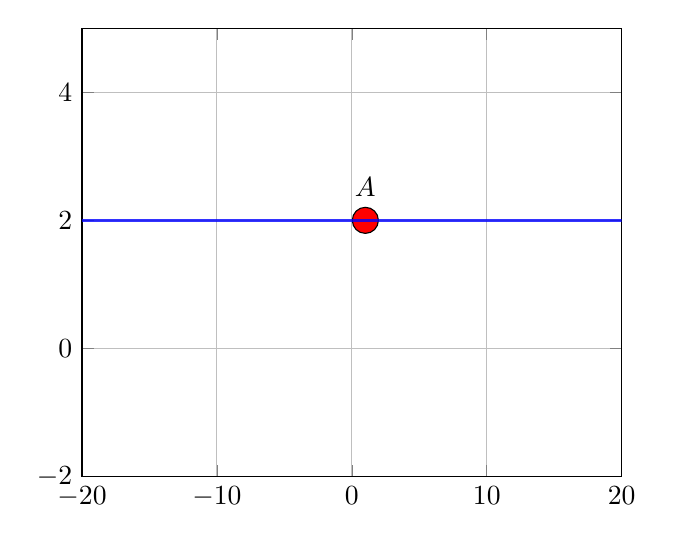
\begin{tikzpicture}[scale=1, transform shape]
    \begin{axis}[xmin=-20,xmax=20,ymin=-2,ymax=5, grid ]
      
    \node[draw,circle, fill=red, label=$A$] at (axis cs:1,2) {};
    \path[draw, very thick, blue, opacity=0.8] (axis cs: -20,2) -- (axis cs: 20,2);
    \end{axis}
  \end{tikzpicture}
  \end{center}
  \caption{ Classe d'équivalence du point $A(1,2)$.}%
  \end{figure}
\end{myproof}

% }}} Exercice 22 %
% Exercice 23 {{{ %
\qs{}
{
\begin{enumerate}
  \item
    Montrer que la relation $\mathcal{R}$ d\'{e}finie sur $\mathbb{R}$ par :
$$x\mathcal{R} y\Longleftrightarrow xe^{y}=ye^{x}$$
est une relation d'\'{e}quivalence.
\item
  Pr\'{e}ciser, pour $x$ fix\'{e} dans $\mathbb{R}$, le nombre d'\'{e}l\'{e}ments de
la classe de $x$ modulo $\mathcal{R}$.
\end{enumerate}
}
\begin{myproof}
Démontrons qu'il s'agit bien d'une relation d'équivalence:  

\begin{itemize}
  \item \textbf{Réflexive}\\
    On as 
    $$
    x e^x = x e^x \implies x\;\mathcal{R}\; x
    $$
  \item \textbf{symétrique}

    Supposons que $x \;\mathcal{R}\; y$ On as alors
    $$ xe^y = y e^x \implies ye^x
    = xe^y \implies y \;\mathcal{R}\; x
    $$
  \item \textbf{Transitive}
    On suppose que 
    $$
    x\;\mathcal{R}\; y \quad \text{ et } \quad y \;\mathcal{R}\; z
    $$
    On aura alors
    $$
    \begin{cases}
      xe^y &= ye^x   \\[2pt]
      ye^z &= ze^y   \\[2pt]
    \end{cases}
    $$
    On multiplies les deux équations (pour $x\ne0$)
    on trouve que 

    $$
    xye^ye^z = zy e^xe^y
    $$
    On obtient alors
    $$
    xe^z = ze^x
    $$
\nt{ pour le cas de $x=0$, aura alors forcement que $y=0$ et $z=0$. Ainsi 
  $$
  x \;\mathcal{R}\; z
  $$
}
\item Soit $x\in \mathbb{R}$ un élément de $\mathbb{R}$ et cherchons sa classe
  d'équivalence.
  % $$
  % $$
  \begin{eqnarray}
    Cl(x) & = &\left\{ y \in \mathbb{R}\;\quad \; xe^y = ye^x\right\}\\
    Cl(x) & = &\left\{ y \in \mathbb{R}\;\quad \; xe^{-x} = ye^{-y}\right\}\\
  \end{eqnarray}
  Ainsi la classe de $x$ est l'ensemble des antécédent de $f(x)$ ou $f(x) =
  xe^{-x}$. Si on représente cette fonction on trouve

  \begin{figure}[htpb]
  \begin{center}
  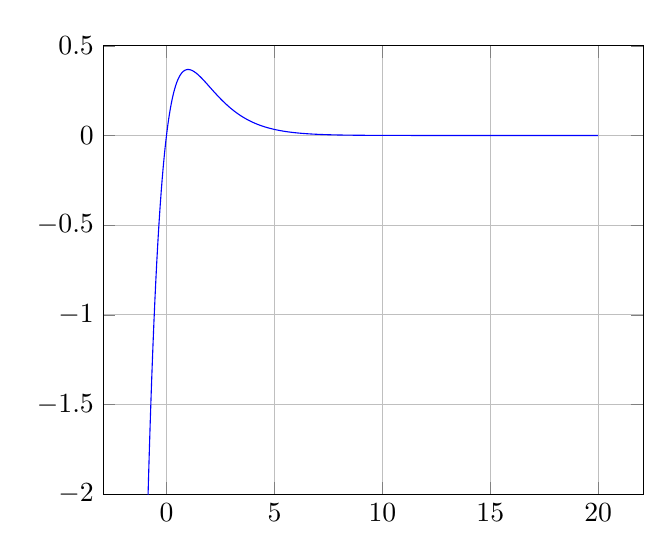
\begin{tikzpicture}[scale=1, transform shape]
    \begin{axis}[grid,ymin=-2,ymax=0.5]
      
  \addplot[blue,domain=-1:20,samples=500] {x*exp(-x) )};
    \end{axis}
    
  \end{tikzpicture}
  \end{center}
  \caption{Graphe de la fonction $xe^{-x}$}%
  \label{fig:}
  \end{figure}
 On remarque depuis le graphe que

 \begin{itemize}
   \item si $x\in ]0,\infty[$ le nombre d'antécédent est $2$.
   \item Pour le reste chaque élément admet un seul antécédent.
 \end{itemize}
\end{itemize}
\end{myproof}

% }}} Exercice 23 %
\newpage

% Execercice 24 {{{ %
\section{Exercice 24}
\qs{}
{
\'Etudier les propri\'et\'es des relations suivantes. Dans le cas
d'une relation d'\'equivalence, pr\'eciser les classes, dans le cas
d'une relation d'ordre, pr\'eciser si elle est totale, si l'ensemble admet
un plus petit ou plus grand \'el\'ement.
\begin{enumerate}
    \item Dans $\mathcal{P}(E)$:
      $$A\;\mathcal{R}_1\; B \iff A\subset B\quad$$

    \item Dans $\mathcal{P}(E)$ $$A\;\mathcal{R}_2\; B \iff A\cap
      B=\emptyset$$
    \item Dans $\mathbb{Z}$:
      $$ a\;\mathcal{R}_3\; b \iff \exists n\in \mathbb{N} \ \,a-b=3n$$
\end{enumerate}
}
\begin{myproof}
  \begin{enumerate}
    \item Demontrons que la premiere relation est une relation d'ordre.
      \begin{enumerate}
        \item \textbf{Reflexive} : $ \forall A \in \mathcal{P}(E), A \subset A
          \implies A\;\mathcal{R}_1\;A$
        \item \textbf{anti-symétrique}: \\
          $$
          \text{si } A \subset B \quad \text{ et } B \subset A \implies A = B
          $$
        \item \textbf{transitive}:
          $$
          \text{ si } A\subset B \;\;\text{ et }\;\; B \subset C \implies A
          \subset C
          $$
          S'agit t'il d'une relation d'ordre totale, \textbf{Non}, car par
          exemple $A=\{1, 2\} $ et $B = \{2, 3\}$, On as 
          $$
          A\not \in B \quad \text{et}\quad B \not\in A
          $$
          Oui la relation admet un petit élément et grand élément

          $$
          \forall A \subset E, \emptyset \subset A\quad \text{et}\quad A \subset
          E.
          $$
      \end{enumerate}
    \item La deuxieme n'est pas une relation car elle n'est pas
      \textbf{réflexive}
      $$
      A \cap A = A \implies \lceil(A \;\mathcal{R}_2\; A)
      $$

\item Démontrons que $\mathcal{R}_3$ est une relation d'ordre.

  \begin{enumerate}
    \item \textbf{Reflexive} : $\forall n \in \mathbb{Z} n - n = 0 = 3\times0
      \implies n \;\mathcal{R}_3\; n$
    \item \textbf{anti-symétrique}: \\
      $$
      \begin{cases}
        a\;\mathcal{R}\;b & \implies \exists n_1 \in \mathbb{N} \quad a - b =
        3n_1\\
        b\;\mathcal{R}\;a &\implies \exists n_2 \in \mathcal{N}\quad b - a =
        3n_2
      \end{cases}
      $$
      On conclut que $n_1 = -n_2 \implies n_1 = n_2 = 0$  Ainsi $$ a= b$$.
    \item  \textbf{transitive}\\
      $$
      \begin{cases}
        a\;\mathcal{R}\;b & \implies \exists n_1 \in \mathbb{N} \quad a - b =
        3n_1\\
        b\;\mathcal{R}\;c &\implies \exists n_2 \in \mathcal{N}\quad b - c =
        3n_2
      \end{cases}
      $$
      Ainsi

      $$
      a - c = 3(\underbrace{n_1+n_2}_{\in \mathbb{N}})
      $$
      Ce qui prouve que 
      $$
      a \;\mathcal{R}\; c
      $$
  \end{enumerate}
  \end{enumerate}
  
\end{myproof}

% }}} Execercice 24 %


% Exercice 25 {{{ %
\section{Exercice 25}
\qs{}
{
Soit $ (E, \leq)$ un ensemble ordonn\'e.\\
On d\'efinit sur $\mathcal{P} (E)\setminus\left\{ \emptyset \right\}$ la relation
$\prec$ par 
$$X \prec Y \quad \text{ ssi } \quad (X = Y \ \text{ ou } \ 
\forall x \in X \  \forall y \in Y \  x \leq y).$$ 
\begin{enumerate}
  \item  V\'erifier que c'est une relation d'ordre.
\end{enumerate}
}
\begin{myproof}
 On démontre qu'il s'agit d'une relation d'ordre. 
 \begin{enumerate}
   \item \textbf{Réflexive}
     $$
     \forall X \subset E\quad X = X \implies X \prec X
     $$
 
   \item \textbf{anti-symétrique}: Soit deux ensembles $X$ et $Y$ tel que $X
     \prec Y$ et $Y \prec X$.
     On note $R(X,Y)$ la deuxième condition:

     $$
     R(X,Y) = \forall x \in X\; \forall y \in Y\; x \leq y
     $$
     Pour le cas d'égalité c'est déjà ce qu'on cherche. Il reste le cas ou on as 
     $$
     R(X,Y) \quad \text{et} \quad R(Y,X)
     $$
     Supposons qu'il existe $x \in X$ tel que $x \not\in Y$. On prend $y \in Y$.
     $$
     \begin{cases}
       R(X,Y) &\implies x \leq y\\ 
       R(Y,X) &\implies y \leq x\\
     \end{cases}
     $$
     \nt{ On peut choisir cet élément car $Y = \emptyset$} 

     On conclut alors que 
     $$
     x = y
     $$
     Ce qui est absurde.
     Ainsi 
     $$
     X = Y
     $$
   \item \textbf{transitive}: Pour trois ensemble $X$, $Y$ et $Z$, on
     suppose qu'on as:
     $$
     X \prec Y \quad \text{ et } \quad Y \prec Z
     $$

     On aura quatre cas:
     

     $$
     \begin{cases}
       X=Y \text{ et } Y = Z & \implies X = Z \implies X \prec Z\\
       X=Y \text{ et } R(Y,Z) & \implies R(X,Z) \implies X\prec Z \\
       R(X,Y) \text{ et } Y = Z & \implies R(X,Z) \implies X \prec Z\\
       R(X,Y) \text{ et } R(Y,Z) & \implies R(X, Z) \implies X \prec Z.
     \end{cases}
     $$
 \end{enumerate}
\end{myproof}

% }}} Exercice 25 %

\end{document}
